\section{Análisis exploratorio y características del dataset} \label{sec:anexo_analisis_exploratorio_caracteristicas_dataset}

\subsection{Exploración de datos de PeeringDB}  \label{sec:anexo_exploracion_datos_peeringdb}





A continuación, se presenta una breve exploración del archivo de peeringDB correspondiente a la fecha de 02/01/2024 
\texttt{peeringdb\_2\_dump\_2024\_02\_01.json}, el cual contiene información pública utilizada para describir la infraestructura de Sistemas Autónomos (ASes), Internet Exchange Points (IXPs) y organizaciones asociadas. \\


El archivo se encuentra en formato \texttt{JSON} y contiene las siguientes claves principales:
\begin{verbatim}
dict_keys(['ixlan', 'ixfac', 'carrierfac', 'netixlan', 'ix', 'net', 
           'netfac', 'poc', 'api', 'fac', 'carrier', 'org', 
           'ixpfx', 'as_set', 'campus'])
\end{verbatim}

Las tablas más importantes para este estudio son las siguientes :
\begin{itemize}
    \item \textbf{net}: Las redes (AS) registradas en PeeringDB, junto con su información  de país, tipo de organización, tráfico e información de peering.
    
    \item \textbf{ix}: Información general de los Internet Exchange Points (IXPs) con su información de nombre, país, ciudad, organización administradora, etc.

    \item \textbf{fac}: Representa las instalaciones o centros de datos donde las redes y los IXPs están físicamente presentes. Incluye información geográfica y de estado operativo.
    
    \item \textbf{netfac}: Relaciona cada red (\textbf{net}) con los centros de datos (\textbf{fac}) en los que tiene presencia.

    \item \textbf{org}: Contiene información sobre las organizaciones administradoras de redes, IXPs y facilities, como su nombre, país y tipo de entidad.

\end{itemize}


\subsubsection*{Exploración de la tabla \texttt{net}}

Esta tabla recopila la información disponible en PeeringDB sobre diferentes Sistemas Autónomos presentes en Internet y que se tiene su registro en dicha plataforma. Cada elemento representa un AS y describe atributos como tipo de organización, tráfico, políticas de peering, características de conectividad entre otras. 
Al transformar esta a un Data Frame, esta contiene \textbf{29,418} filas correspondiente a información sobre diferentes ASes y \textbf{40} columnas correspondiente a atributos de estos.\\

En primer lugar, se analizaron las columnas y sus tipos de datos, identificando \textbf{6 columnas numéricas}, \textbf{27 categóricas} y \textbf{6 booleanas}.


\begin{lstlisting}[language=Python, caption={Columnas del conjunto de datos \texttt{net}.}, label={lst:columnas_net}]
=== Columnas numéricas ===
['fac_count', 'id', 'ix_count', 'org_id', 'info_prefixes6', 'info_prefixes4']

=== Columnas categóricas ===
['status', 'looking_glass', 'route_server', 'netixlan_updated', 'info_ratio', 
 'status_dashboard', 'rir_status', 'created', 'name_long', 'policy_general', 
 'website', 'updated', 'info_types', 'rir_status_updated', 'netfac_updated', 
 'info_traffic', 'policy_locations', 'name', 'info_scope', 'notes', 'policy_url', 
 'poc_updated', 'info_type', 'social_media', 'policy_contracts', 'aka', 'irr_as_set']

=== Columnas booleanas ===
['policy_ratio', 'info_unicast', 'allow_ixp_update', 'info_multicast', 
 'info_never_via_route_servers', 'info_ipv6']
\end{lstlisting}


Tras esta primera exploración, se decidió conservar las columnas categóricas relevantes para el estudio, principalmente aquellas que entregan información sobre políticas de conexión, tráfico y alcance de red. Las categorías identificadas se resumen en la Tabla~\ref{tab:categorias_peeringdb_clara}.




\begin{table}[H]
\centering
\caption{Resumen de las categorías presentes en las columnas categóricas seleccionadas del conjunto \texttt{net} de PeeringDB.}
\label{tab:categorias_peeringdb_clara}
\begin{tabularx}{\textwidth}{lX}
\hline
\textbf{Columna} & \textbf{Categorías y ejemplos de valores} \\
\hline

\texttt{policy\_contracts} (4 categorías) &
Required, Not Required, Private Only, (vacío). \\

\texttt{info\_type} (10 categorías) &
NSP, Content, Non-Profit, Cable/DSL/ISP, Educational/Research, 
Network Services, Enterprise, Route Server, Route Collector, (vacío). \\

\texttt{info\_scope} (11 categorías) &
Global, Europe, North America, Regional, Asia Pacific, South America, 
Not Disclosed, Australia, Middle East, Africa, (vacío). \\

\texttt{policy\_locations} (6 categorías) &
Required – International, Not Required, Preferred, Required – US, Required – EU, (vacío). \\

\texttt{info\_traffic} (19 categorías) &
0–20 Mbps, 20–100 Mbps, 5–10 Gbps, 10–20 Gbps, 100–200 Gbps, 500–1000 Gbps, 
1–5 Tbps, 50–100 Tbps, 100+ Tbps, (vacío). \\

\texttt{info\_types} (9 categorías) &
NSP, Content, Non-Profit, Cable/DSL/ISP, Educational/Research, 
Network Services, Enterprise, Route Server, Route Collector. \\

\texttt{policy\_general} (5 categorías) &
Restrictive, Open, Selective, No, (vacío). \\

\texttt{info\_ratio} (7 categorías) &
Balanced, Heavy Inbound, Heavy Outbound, Mostly Inbound, 
Mostly Outbound, Not Disclosed, (vacío). \\

\hline
\end{tabularx}
\end{table}



Posteriormente, se analizó los valores faltantes en las distintas columnas.  
En el caso de las columnas numéricas, se consideraron faltantes los valores \texttt{NaN} y aquellos igual a cero (Tabla~\ref{tab:faltantes_numericos}).


\begin{table}[H]
\centering
\caption{Porcentaje de valores faltantes o nulos en columnas numéricas del conjunto \texttt{net}.}
\label{tab:faltantes_numericos}
\begin{tabular}{lcc}
\hline
\textbf{Columna} & \textbf{Faltantes} & \textbf{\% Faltantes} \\
\hline
\texttt{fac\_count}       & 17,617 & 59.89 \\
\texttt{ix\_count}        & 14,077 & 47.85 \\
\texttt{info\_prefixes6}  & 11,870 & 40.35 \\
\texttt{info\_prefixes4}  & 9,107  & 30.96 \\
\texttt{id}               & 0      & 0.00 \\
\texttt{org\_id}          & 0      & 0.00 \\
\hline
\end{tabular}
\end{table}

De igual forma para las columnas categóricas s consideraron como faltantes los valores \texttt{NaN} y los string vacios. Los resultados se muestran en la Tabla~\ref{tab:faltantes_categoricas}.

\begin{table}[H]
\centering
\caption{Porcentaje de valores faltantes en las columnas categóricas seleccionadas del conjunto \texttt{net} de PeeringDB.}
\label{tab:faltantes_categoricas}
\renewcommand{\arraystretch}{1.2}
\begin{tabular}{lcc}
\hline
\textbf{Columna} & \textbf{Faltantes} & \textbf{\% Faltantes} \\
\hline
\texttt{info\_traffic}      & 12,047 & 40.95 \\
\texttt{info\_type}         & 8,439  & 28.69 \\
\texttt{policy\_contracts}  & 1,462  & 4.97  \\
\texttt{policy\_general}    & 1,352  & 4.60  \\
\texttt{policy\_locations}  & 1,353  & 4.60  \\
\texttt{info\_ratio}        & 663    & 2.25  \\
\texttt{info\_scope}        & 370    & 1.26  \\
\texttt{info\_types}        & 0      & 0.00  \\
\hline
\end{tabular}
\end{table}


Finalmente, la Tabla~\ref{tab:categorias_categoricas} resume las columnas categóricas seleccionadas junto con el número de categorías únicas y algunos ejemplos representativos.  
Este resumen permite identificar de forma clara la diversidad de información contenida en PeeringDB y la relevancia de cada atributo para su posterior uso en la construcción de modelos basados en grafos.


\begin{table}[H]
\centering
\caption{Resumen de columnas categóricas y número de categorías únicas en PeeringDB.}
\label{tab:categorias_categoricas}
\begin{tabular}{lcc}
\hline
\textbf{Columna} & \textbf{Categorías únicas} & \textbf{Ejemplos de categorías} \\
\hline
policy\_general & 5 & Open, Selective, Restrictive, No \\
info\_type & 10 & NSP, Content, Non-Profit, Enterprise, Route Server \\
info\_scope & 11 & Global, Europe, North America, Regional, Asia Pacific \\
policy\_locations & 6 & Required - US, Required - EU, Not Required \\
info\_traffic & 18 & 1-5Gbps, 100-200Gbps, 10-20Tbps, 0-20Mbps \\
info\_ratio & 7 & Balanced, Heavy Inbound, Mostly Outbound \\
\hline
\end{tabular}
\end{table}





A continuación, algunas figuras para entender los datos.\\





\begin{figure}[H]
    \centering
    % === 1ra fila ===
    \begin{subfigure}[b]{0.48\textwidth}
        \centering
        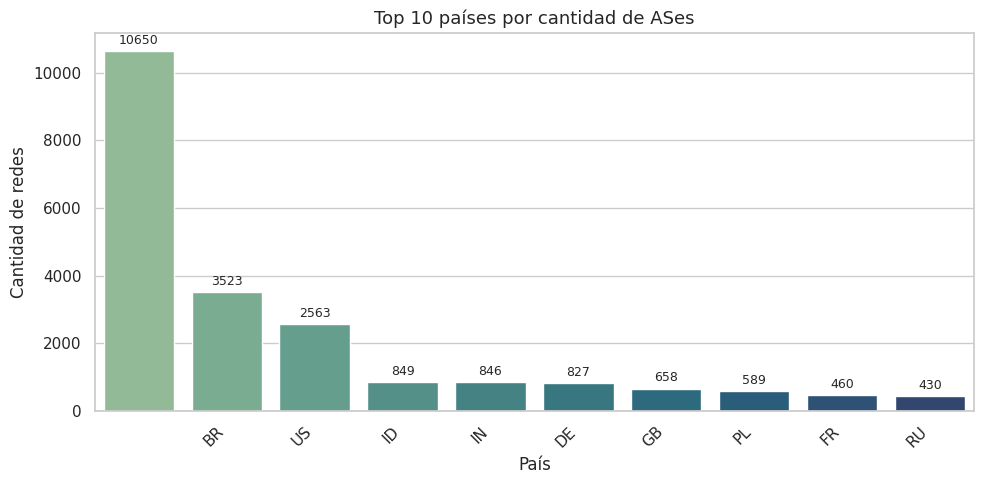
\includegraphics[width=\textwidth]{img/anexoPeeringDB/Top_10_países_por_cantidad_de_ASes.png}
        \caption{Top 10 países con mayor cantidad de ASes registrados en PeeringDB.}
        \label{fig:Top_10_países_por_cantidad_de_ASes}
    \end{subfigure}
    \hfill
    \begin{subfigure}[b]{0.48\textwidth}
        \centering
        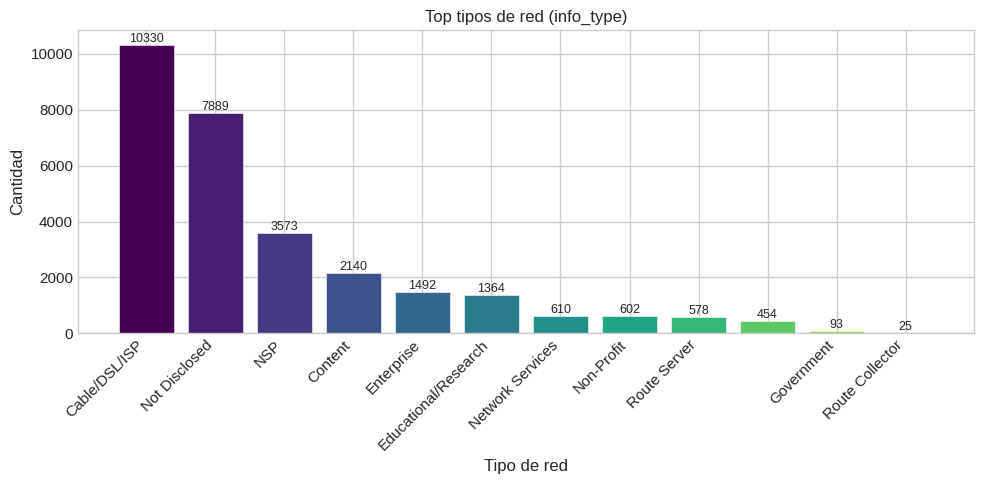
\includegraphics[width=\textwidth]{img/anexoPeeringDB/Top_tipos_de_red_info_type.png}
        \caption{Top tipos de red (\texttt{info\_type}) en ASes registrados en PeeringDB.}
        \label{fig:Top_tipos_de_red_info_type}
    \end{subfigure}

    % === 2da fila ===
    \vspace{5mm}
    \begin{subfigure}[b]{0.48\textwidth}
        \centering
        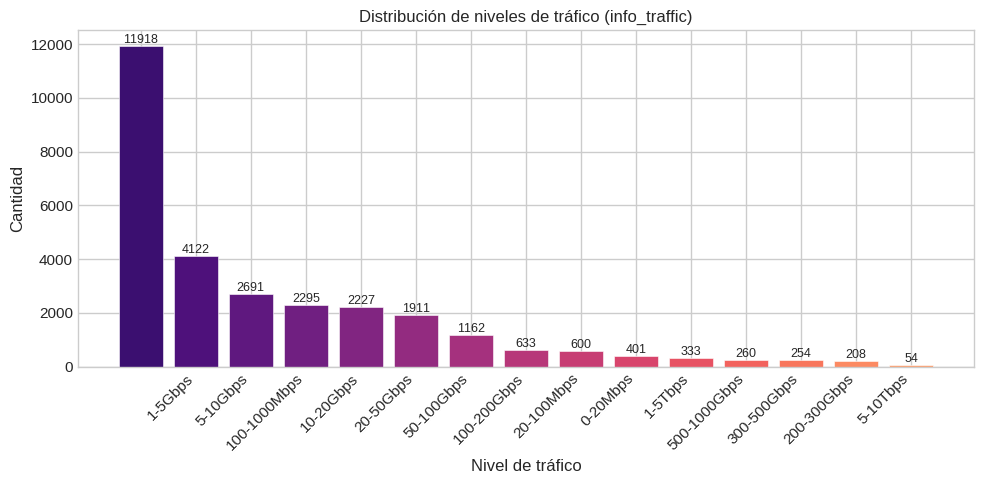
\includegraphics[width=\textwidth]{img/anexoPeeringDB/Distribución_de_niveles_de_tráfico_info_traffic.png}
        \caption{Distribución de niveles de tráfico (\texttt{info\_traffic}).}
        \label{fig:Distribución_de_niveles_de_tráfico_info_traffic}
    \end{subfigure}
    \hfill
    \begin{subfigure}[b]{0.48\textwidth}
        \centering
        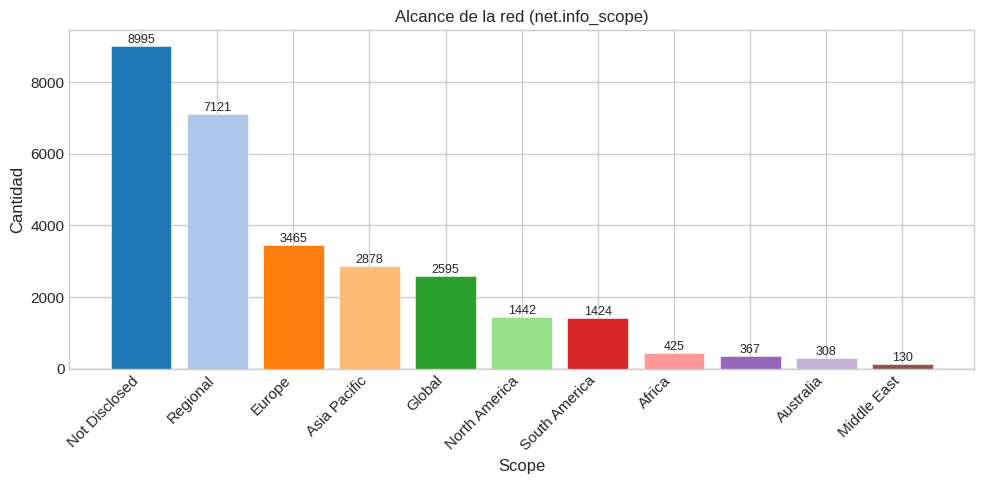
\includegraphics[width=\textwidth]{img/anexoPeeringDB/Alcance_de_la_red_info_scope.png}
        \caption{Alcance de la red (\texttt{info\_scope}).}
        \label{fig:Alcance_de_la_red_info_scope}
    \end{subfigure}

    % === 3ra fila ===
    \vspace{5mm}
    \begin{subfigure}[b]{0.48\textwidth}
        \centering
        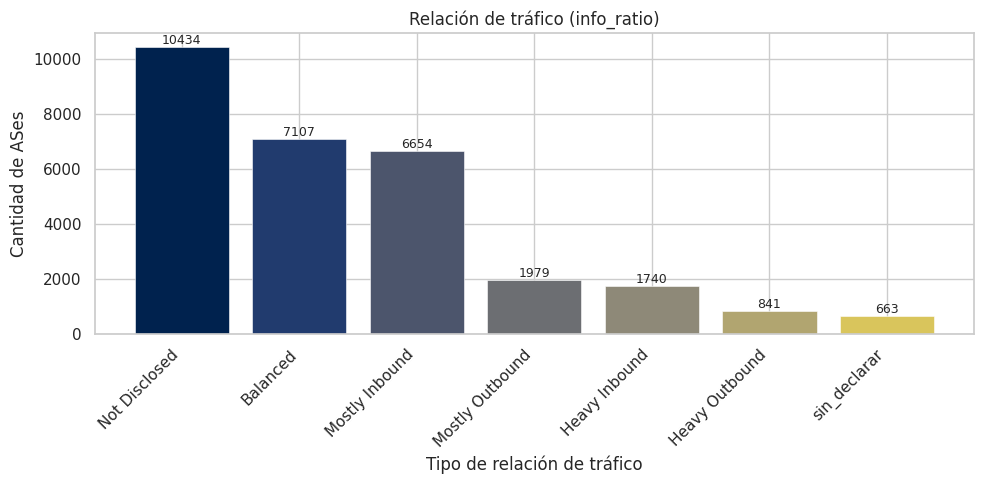
\includegraphics[width=\textwidth]{img/anexoPeeringDB/Relación_de_traficoinfo_ratio.png}
        \caption{Relación de tráfico (\texttt{info\_ratio}).}
        \label{fig:Relación_de_traficoinfo_ratio}
    \end{subfigure}
    \hfill
    \begin{subfigure}[b]{0.48\textwidth}
        \centering
        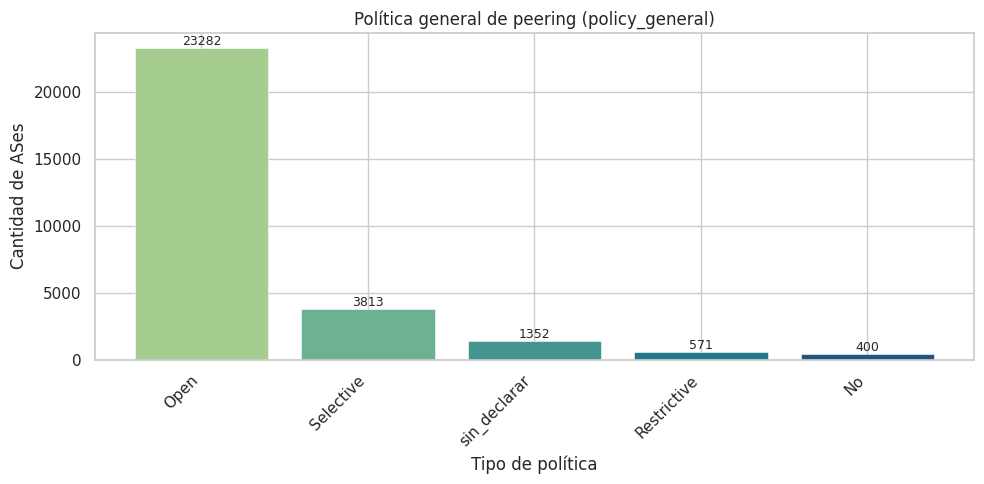
\includegraphics[width=\textwidth]{img/anexoPeeringDB/Politica_general_de_peering_policy_general.png}
        \caption{Política general de peering (\texttt{policy\_general}).}
        \label{fig:Politica_general_de_peering_policy_general}
    \end{subfigure}

    % === 4ta fila ===
    \vspace{5mm}
    \begin{subfigure}[b]{0.48\textwidth}
        \centering
        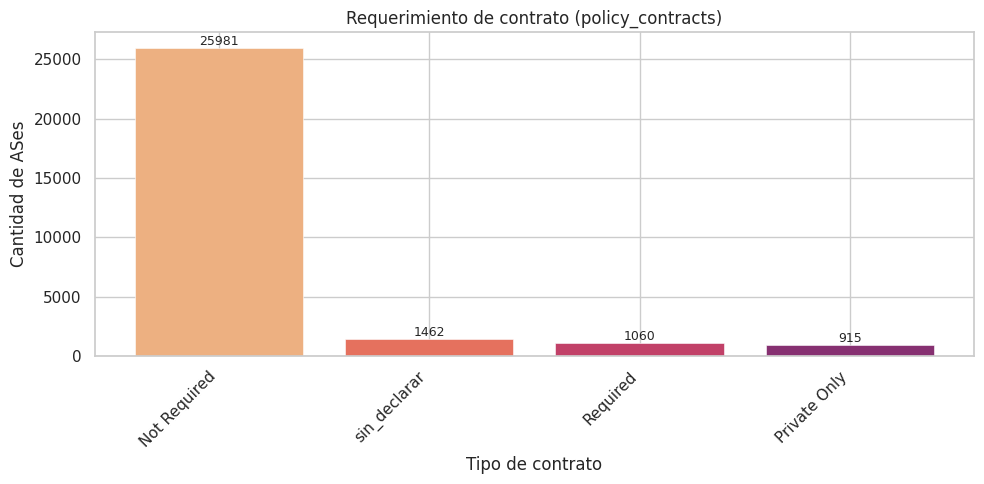
\includegraphics[width=\textwidth]{img/anexoPeeringDB/Requerimiento_de_contrato_policy_contracts.png}
        \caption{Requerimiento de contrato (\texttt{policy\_contracts}).}
        \label{fig:Requerimiento_de_contrato_policy_contracts}
    \end{subfigure}
    \hfill
    \begin{subfigure}[b]{0.48\textwidth}
        \centering
        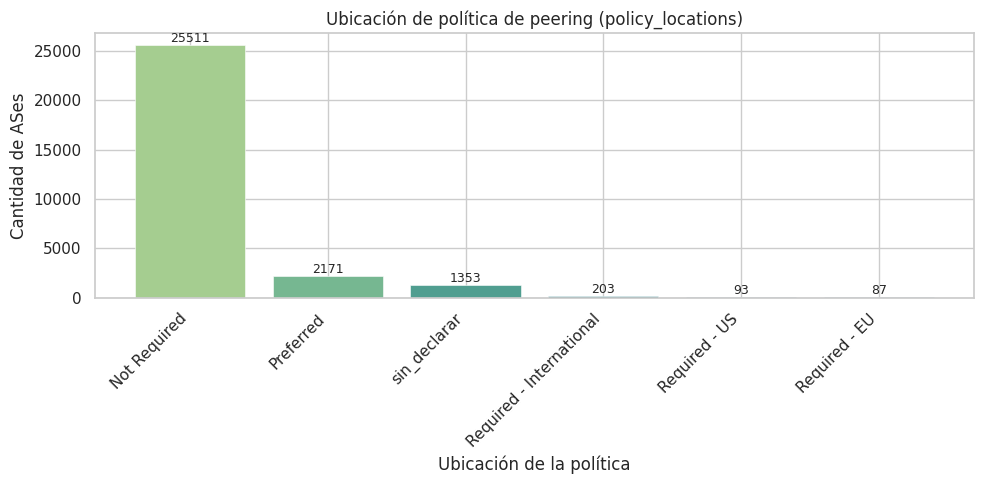
\includegraphics[width=\textwidth]{img/anexoPeeringDB/Ubicacion_de_política_de_peering_policy_locations.png}
        \caption{Ubicación de política de peering (\texttt{policy\_locations}).}
        \label{fig:Ubicacion_de_política_de_peering_policy_locations}
    \end{subfigure}


    \caption{Visualización general de las principales variables categóricas y numéricas del conjunto \texttt{net} de PeeringDB.}
    \label{fig:graficos_peeringdb_completo}
\end{figure}







\begin{figure}[H]
    \centering
    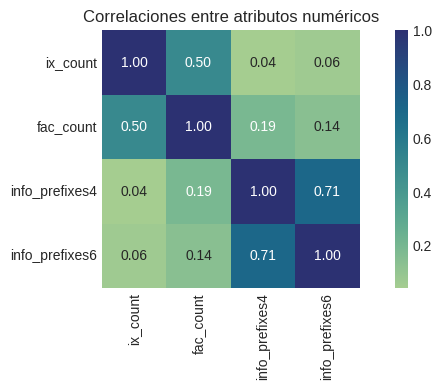
\includegraphics[width=0.6\textwidth]{img/anexoPeeringDB/Correlaciones_entre_atributos_numericos.png}
    \caption{Matriz de correlación entre los atributos numéricos extraidos de PeeringDB.}
    \label{fig:Correlaciones_entre_atributos_numericos}
\end{figure}

Con la visualización de la Figura~\ref{fig:Correlaciones_entre_atributos_numericos} podemos decir:
\begin{itemize}
    \item los AS que anuncian muchos prefijos IPv4 tienden también a anunciar muchos prefijos IPv6. Puedes esperar colinealidad entre ambos.
    \item más IXPs suele venir acompañado de presencia en más facilities (tamaño/cobertura del AS).
\end{itemize}



\begin{table}[H]
\centering
\caption{Porcentaje de filas sin información por columna (antes de limpieza).}
\label{tab:faltantes_net}
\begin{tabular}{l l r r}
\toprule
\textbf{columna} & \textbf{tipo} & \textbf{sin\_info} & \textbf{porcentaje \%} \\
\midrule
info\_traffic      & categórica & 12047 & 40.95 \\
info\_type         & categórica & 8439  & 28.69 \\
policy\_contracts  & categórica & 1462  & 4.97  \\
policy\_general    & categórica & 1352  & 4.60  \\
policy\_locations  & categórica & 1353  & 4.60  \\
info\_ratio        & categórica & 663   & 2.25  \\
info\_scope        & categórica & 370   & 1.26  \\
info\_prefixes4    & numérica   & 0     & 0.00  \\
fac\_count         & numérica   & 0     & 0.00  \\
ix\_count          & numérica   & 0     & 0.00  \\
info\_prefixes6    & numérica   & 0     & 0.00  \\
\bottomrule
\end{tabular}
\end{table}



\subsection{Atributos numéricos}
\label{subsec:attr_num_peeringdb}

La Figura~\ref{fig:attr_num_peeringdb} muestra la distribución de cuatro atributos numéricos provenientes de PeeringDB, tras aplicar el preprocesamiento definido (transformación logarítmica y normalización min--max a $[0,1]$). Para cada atributo se incluye además la media (línea roja) y la mediana (línea azul), con el fin de evidenciar asimetrías y posibles valores extremos.

\begin{figure}[H]
    \centering
    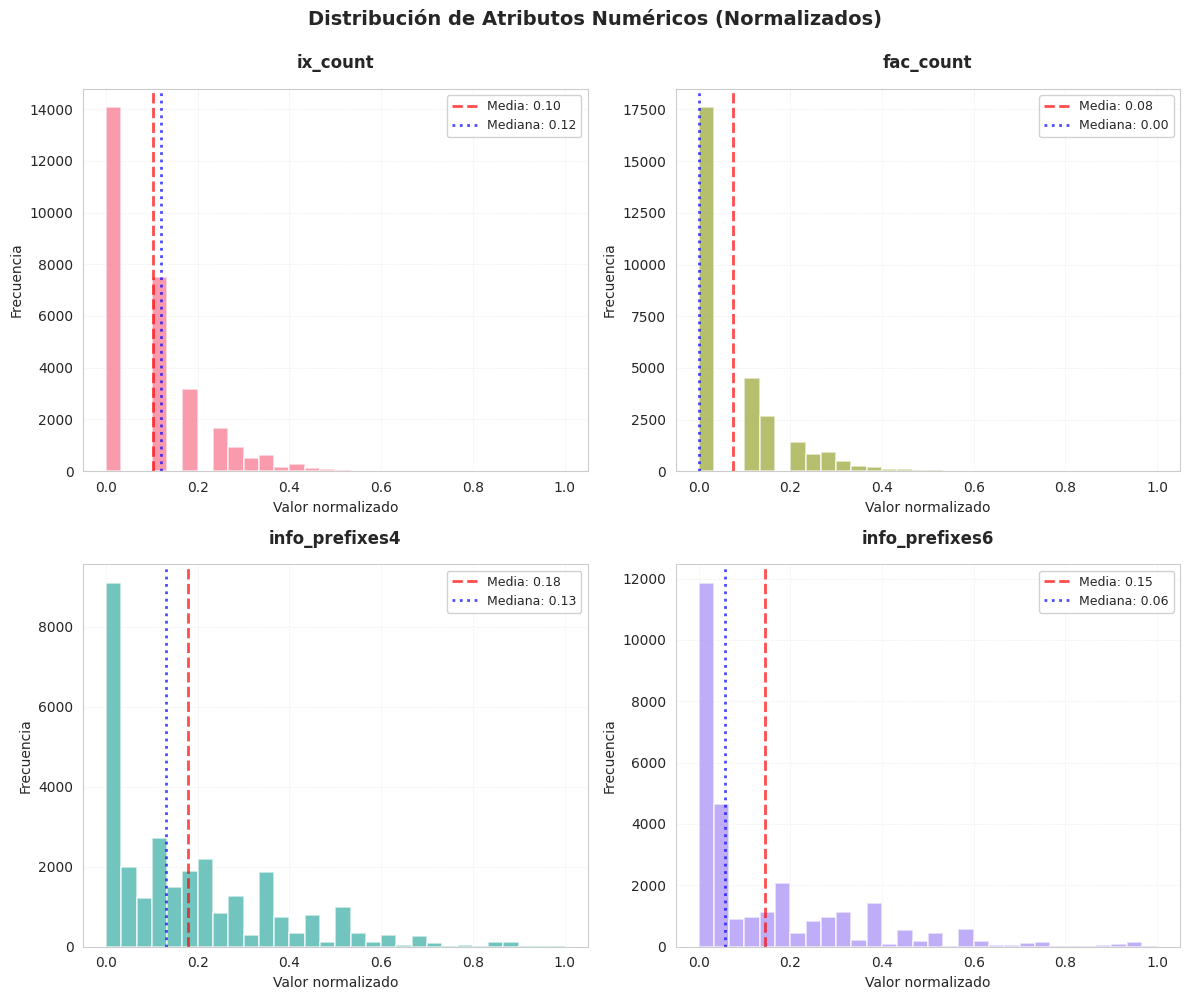
\includegraphics[width=0.85\linewidth]{Anexos/attr_num_peeringdb.png}
    \caption{Distribución de atributos numéricos de PeeringDB normalizados ($[0,1]$). Se muestran \texttt{ix\_count}, \texttt{fac\_count}, \texttt{info\_prefixes4} e \texttt{info\_prefixes6}, junto con la media (rojo) y la mediana (azul).}
    \label{fig:attr_num_peeringdb}
\end{figure}

\paragraph{Media vs.\ mediana: sesgo y presencia de outliers.}
En general, la media se ubica a la derecha de la mediana (media $>$ mediana), lo cual es consistente con distribuciones con \emph{cola derecha}. Esto sugiere la presencia de pocos AS con valores muy altos (outliers) que elevan la media, mientras que la mayoría de los AS se concentra en valores bajos.

\paragraph{Comparación entre atributos.}
\begin{itemize}
    \item \textbf{\texttt{ix\_count}:} la mayoría de los AS participa en pocos IXPs, y existe un grupo reducido con participación en muchos IXPs.
    \item \textbf{\texttt{fac\_count}:} la distribución está fuertemente concentrada cerca de 0; muchos AS reportan pocas (o ninguna) facilities, y pocos AS acumulan un número alto.
    \item \textbf{\texttt{info\_prefixes4} y \texttt{info\_prefixes6}:} muestran mayor variabilidad y una cola larga; un conjunto pequeño de AS anuncia muchos prefijos, mientras que la mayoría anuncia pocos.
\end{itemize}

\paragraph{Efecto del preprocesamiento (log + min--max).}
Aunque los atributos fueron normalizados a $[0,1]$, las distribuciones permanecen ``pegadas'' a 0. Esto indica que, incluso tras la transformación logarítmica, la mayoría de los AS mantiene valores pequeños en comparación con el máximo observado. Este comportamiento es típico en redes reales, donde coexisten pocos AS muy grandes (p.\,ej., backbone/tier-1 o redes altamente conectadas) y una gran cantidad de AS pequeños.

\paragraph{Implicancias para el modelado.}
Estas distribuciones sugieren que:
\begin{itemize}
    \item existen \textbf{outliers potencialmente relevantes} (AS muy grandes),
    \item la \textbf{mediana} describe mejor al AS ``típico'' que la media,
    \item podría ser útil evaluar alternativas robustas si el modelo es sensible a extremos (p.\,ej., \emph{RobustScaler}, winsorización o clipping por percentiles).
\end{itemize}




\subsubsection{Atributos categóricos}
\label{subsec:attr_cat_peeringdb}

La Figura~\ref{fig:attr_cat_peeringdb} muestra la distribución de atributos categóricos extraídos desde PeeringDB. En general, se observa un marcado \textbf{desbalance de clases} en la mayoría de variables, con categorías dominantes (muy frecuentes) y un conjunto de categorías raras con baja representación. Este patrón es relevante porque impacta directamente en la representación mediante \emph{one-hot encoding} (alta esparsidad) y en la contribución efectiva de cada atributo al modelo.

\begin{figure}[H]
    \centering
    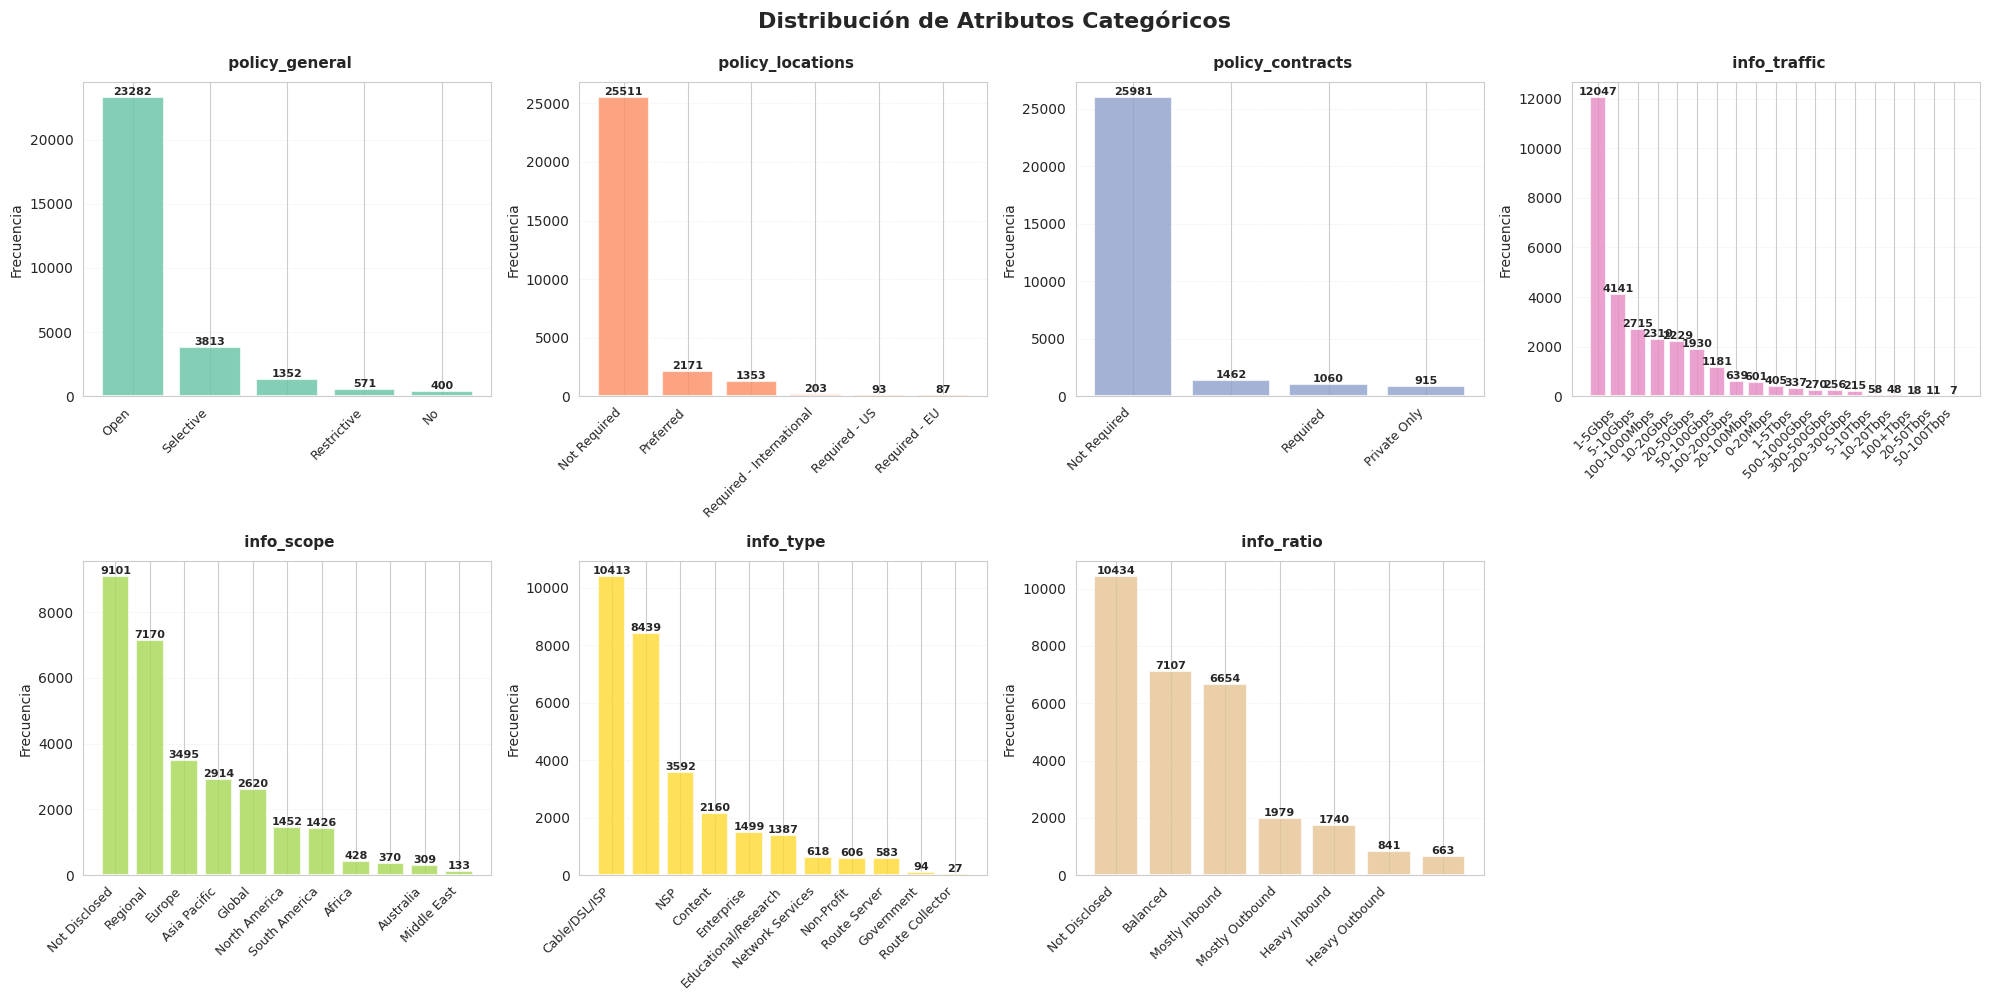
\includegraphics[width=0.95\linewidth]{Anexos/attr_cat_peeringdb.png}
    \caption{Distribución de atributos categóricos de PeeringDB. Se muestran variables de política (\texttt{policy\_general}, \texttt{policy\_locations}, \texttt{policy\_contracts}) e información declarada (\texttt{info\_traffic}, \texttt{info\_scope}, \texttt{info\_type}, \texttt{info\_ratio}).}
    \label{fig:attr_cat_peeringdb}
\end{figure}

\paragraph{Variables de política (\texttt{policy\_general}, \texttt{policy\_locations}, \texttt{policy\_contracts}).}
En \texttt{policy\_general} predomina ampliamente \emph{Open}, seguida a distancia por \emph{Selective}, mientras que \emph{Restrictive} y \emph{No} aparecen con baja frecuencia. De forma similar, en \texttt{policy\_locations} y \texttt{policy\_contracts} domina \emph{Not Required}, y las categorías que implican requisitos específicos (\emph{Required} por región o condiciones) son minoritarias. En conjunto, estas distribuciones sugieren que la mayoría de los AS no declara restricciones fuertes, por lo que estas variables quedan representadas por pocas categorías con alta concentración.

\paragraph{\texttt{info\_traffic}.}
Esta variable presenta una distribución con muchas categorías y una caída rápida en frecuencia: predominan rangos bajos/medios, mientras que los rangos altos aparecen con muy pocos casos. Aunque se presenta como categórica, su naturaleza es más cercana a una variable \textbf{ordinal} (rangos de tráfico), por lo que su representación puede beneficiarse de estrategias que respeten el orden (en vez de tratar cada categoría como independiente).

\paragraph{\texttt{info\_scope}.}
Las categorías más frecuentes corresponden a \emph{Not Disclosed} y \emph{Regional}, seguidas por categorías geográficas (p.\,ej., \emph{Europe}, \emph{Asia Pacific}, etc.) con menor presencia. La alta proporción de \emph{Not Disclosed} indica falta de información declarada, lo cual puede interpretarse como una señal informativa en sí misma y conviene conservarla explícitamente como categoría.

\paragraph{\texttt{info\_type}.}
Predominan \emph{Cable/DSL/ISP} y \emph{NSP}, mientras que tipos como \emph{Government}, \emph{Route Collector} u otras categorías aparecen rara vez. Esto sugiere que el atributo está dominado por perfiles de red típicos (ISP/NSP), y que las clases minoritarias podrían aportar poca señal estable si no se tratan adecuadamente.

\paragraph{\texttt{info\_ratio}.}
Se observa nuevamente una alta frecuencia de \emph{Not Disclosed}, seguida por \emph{Balanced} y \emph{Mostly Inbound}. Las categorías extremas (p.\,ej., \emph{Heavy Inbound/Outbound}) son poco frecuentes, reforzando el patrón de desbalance y de información no declarada.

\subsubsection{Implicancias para el preprocesamiento y el modelado}
A partir de estas distribuciones, se desprenden implicancias prácticas:
\begin{itemize}
    \item Varias variables presentan \textbf{categorías dominantes} y múltiples categorías raras, por lo que el \emph{one-hot encoding} generará columnas con muy pocos ``1'' (alta esparsidad).
    \item Puede ser útil \textbf{agrupar categorías infrecuentes} en una clase \emph{Other} (usando un umbral de frecuencia) para reducir dimensionalidad y ruido.
    \item Dado que \texttt{info\_traffic} es esencialmente ordinal, se puede evaluar una \textbf{codificación ordinal} (o mapeo a rangos numéricos) en lugar de one-hot.
    \item Mantener \emph{Not Disclosed} como categoría explícita es recomendable, ya que captura \textbf{ausencia de información declarada}, lo cual puede correlacionarse con el tipo/rol del AS.
\end{itemize}




\subsubsection*{Exploración de Internet Exchange Points}
A modo de contexto, también se incluyen visualizaciones relacionadas con IXPs.

\begin{figure}[H]
    \centering
    % === 1ra fila: dos figuras lado a lado ===
    \begin{subfigure}[b]{0.48\textwidth}
        \centering
        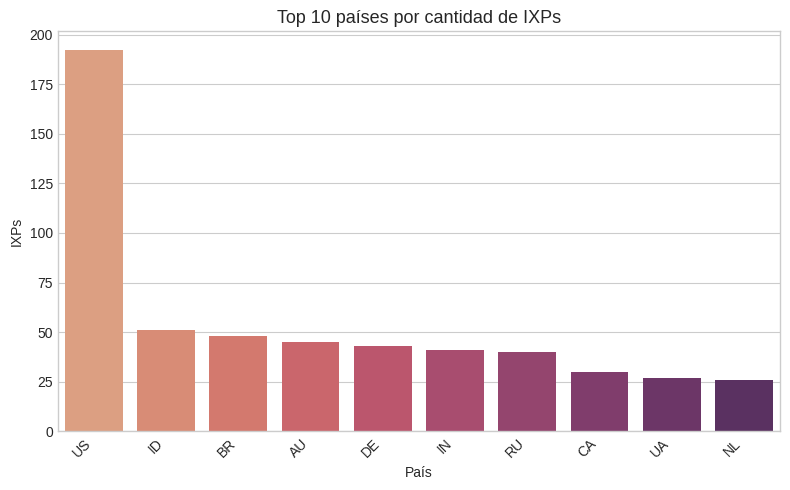
\includegraphics[width=\textwidth]{img/anexoPeeringDB/Top_10_países_por_cantidad_deI_XPs.png}
        \caption{Top 10 países con mayor cantidad de IXPs registrados en PeeringDB.}
        \label{fig:Top_10_países_por_cantidad_deI_XPs}
    \end{subfigure}
    \hfill
    \begin{subfigure}[b]{0.48\textwidth}
        \centering
        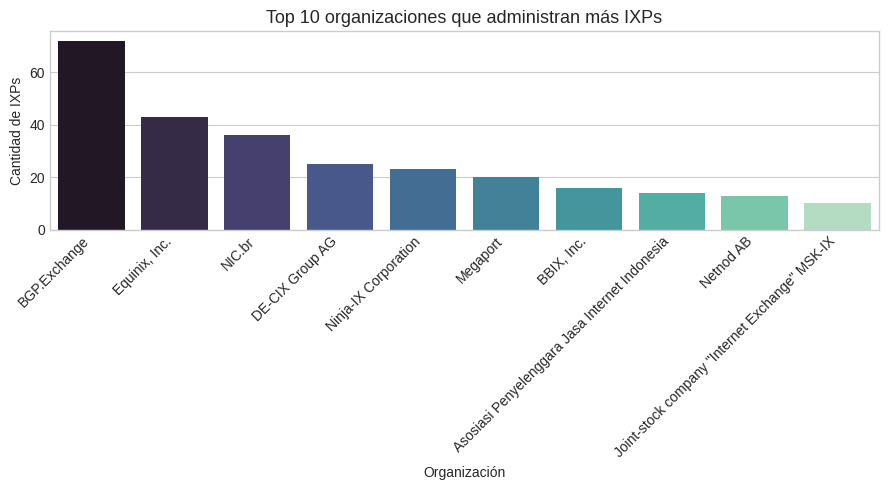
\includegraphics[width=\textwidth]{img/anexoPeeringDB/Top _10_organizaciones_que_administran_mas_IXPs.png}
        \caption{Top organizaciones que administran mayor cantidad de IXPs registrados en PeeringDB.}
        \label{fig:Top_10_org_por_cantidad_deI_XPs}
    \end{subfigure}

    % === 2da fila: figura centrada ===
    \vspace{6mm}
    \begin{subfigure}[b]{0.6\textwidth}
        \centering
        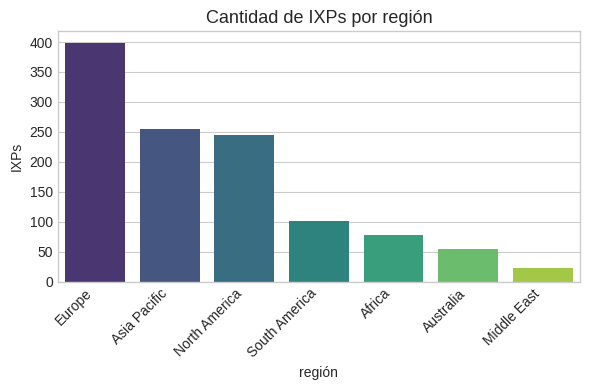
\includegraphics[width=\textwidth]{img/anexoPeeringDB/Cantida_de_IXPs_por_region.png}
        \caption{Cantidad de IXPs por región.}
        \label{fig:Cantida_de_IXPs_por_region}
    \end{subfigure}

    % === Caption general ===
    \caption{Distribución y administración de IXPs registrados en PeeringDB: comparación por país, organización y región geográfica.}
    \label{fig:ixps_peeringdb}
\end{figure}



\begin{table}
\caption{IXPs registrados en Chile según PeeringDB (2024).}
\label{tab:ixps_chile}
\begin{tabular}{l l c}
\toprule
Nombre del IXP & Ciudad & País \\
\midrule
PIT Santiago - PIT Chile & Santiago & CL \\
SCL-IX Chile & Santiago & CL \\
PIT Concepcion - PIT Chile & Concepcion & CL \\
PIT Osorno - PIT Chile & Osorno & CL \\
PIT Temuco - PIT Chile & Temuco & CL \\
PIT Arica - PIT Chile & Arica & CL \\
PIT entel & Santiago & CL \\
BGP.Exchange - Valdivia & Valdivia & CL \\
BGP.Exchange - Santiago & Santiago & CL \\
\bottomrule
\end{tabular}
\end{table}

\section{Tabla Resumen Atributos de ASes de 
trabajo~\cite{BenchmarkingGNN} }

\begin{figure}[h!] % h! = aquí preferentemente
    \centering
    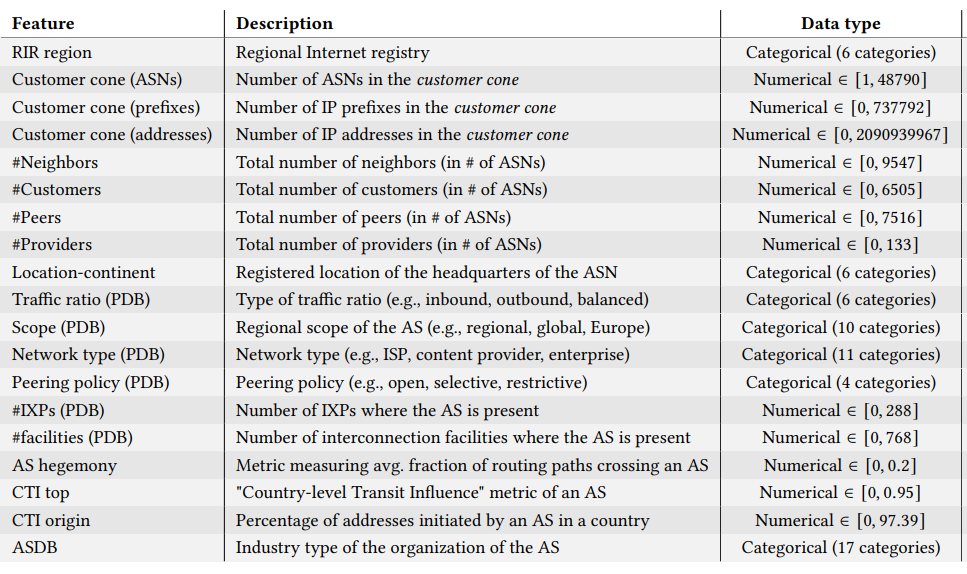
\includegraphics[width=0.9\textwidth]{img/metodologia/tabalAtributosgnnbchn.png}
    \caption{Tabla resumen de atributos del paper ``\textit{Benchmarking Graph Neural Networks for Internet Routing Data}''.}
    \label{tab:as_attr_tabla_bechmark}
\end{figure}



\subsection{Atributos de Sistemas Autónomos utilizados}


\subsection{Análisis de atributos extraídos desde PeeringDB}
Atributos numéricos
Atributos categóricos
\subsection{Análisis del grafo construido}
Grado de salida en datos RIBs
Cantidad de ASes y enlaces en el dataset



\subsection{Análisis temporal de rutas BGP} 







\subsection{Análisis temporal de rutas BGP}
Comparación mensual de longitud de rutas
\subsection{Lista de Sistemas Autónomos Tier-1 considerados}

% TODO: Verificar los Ases esten bien
\begin{table}[ht]
%\centering
\rowcolors{2}{grayA}{grayB}  % ← intercalado entre grisA y grisB

\begin{tabular}{|c|c|c|}
\hline
\textbf{Nombre} & \textbf{Numero} & \textbf{Ubicacion} \\
\hline
Cogent Communications & 174 & Estados Unidos \\
Zayo Group  & 6461 &   Estados Unidos\\
Verizon Enterprise Solutions  & 701 &   Estados Unidos\\
Arelion & 1299 &   Suecia\\
PCCW Global & 3491 & Hong Kong\\
Deutsche Telekom Global Carrier &  	3320 & Alemania\\
Telecom Italia Sparkle & 6762 & Italia\\
AT\&T & 7018 & Estados Unidos\\
Telxius & 12956 &   España\\
Liberty Global & 6830 & Países Bajos\\
Tata Communications & 6453 & India\\
Orange & 5511 & Francia\\
Lumen Technologies & 3356 & Estados Unidos\\
GTT Communications & 3257 &   Estados Unidos\\
NTT Communications & 2914 & Japón\\
Verizon Business & 2828 & Estados Unidos \\
SprintLink & 1239 & Estados Unidos \\
KPN & 286 & Estados Unidos \\
CenturyLink & 209 & Estados Unidos \\
\hline
\end{tabular}
\caption{Lista con Sistemas Autonomos Tier 1}
\label{tab:tier_1_ases}
\end{table}





\subsection{Tabla colectors disponible de RouteViews Project}

\begin{table}[ht]
%\centering
\rowcolors{2}{grayA}{grayB}  % ← intercalado entre grisA y grisB


% FIXME: ARREGLAR TABLA
\begin{tabular}{|c|c|c|}
\hline
\textbf{Nombre} & \textbf{Numero} & \textbf{Ubicacion} \\
\hline
- & - & - \\
- & - & - \\
- & - & - \\
- & - & - \\
\hline
\end{tabular}
\caption{Tabla colectors disponible de RouteViews Project}
\label{tab:tabla_colectors_routeviews}

\end{table}





\subsection{Tabla colectors disponible de RIPE RIS}

% FIXME: Arreglar tabla
\begin{table}[ht]
%\centering
\rowcolors{2}{grayA}{grayB}  % ← intercalado entre grisA y grisB

\begin{tabular}{|c|c|c|}
\hline
\textbf{Nombre} & \textbf{Numero} & \textbf{Ubicacion} \\
\hline
- & - & - \\
- & - & - \\
- & - & - \\
- & - & - \\
- & - & - \\
\hline
\end{tabular}
\caption{Tabla Colectors RIPE RIS}
\label{tab:tabla_colectors_ripe_ris}
\end{table}

------------------











Nose donde poner estas figuras 



Figura~\ref{fig:top_20_as_febrero_numerorelaciones_src} complementaria que presenta el top 20 de ASes según su grado de salida. 

\begin{figure}[H]
    \centering
    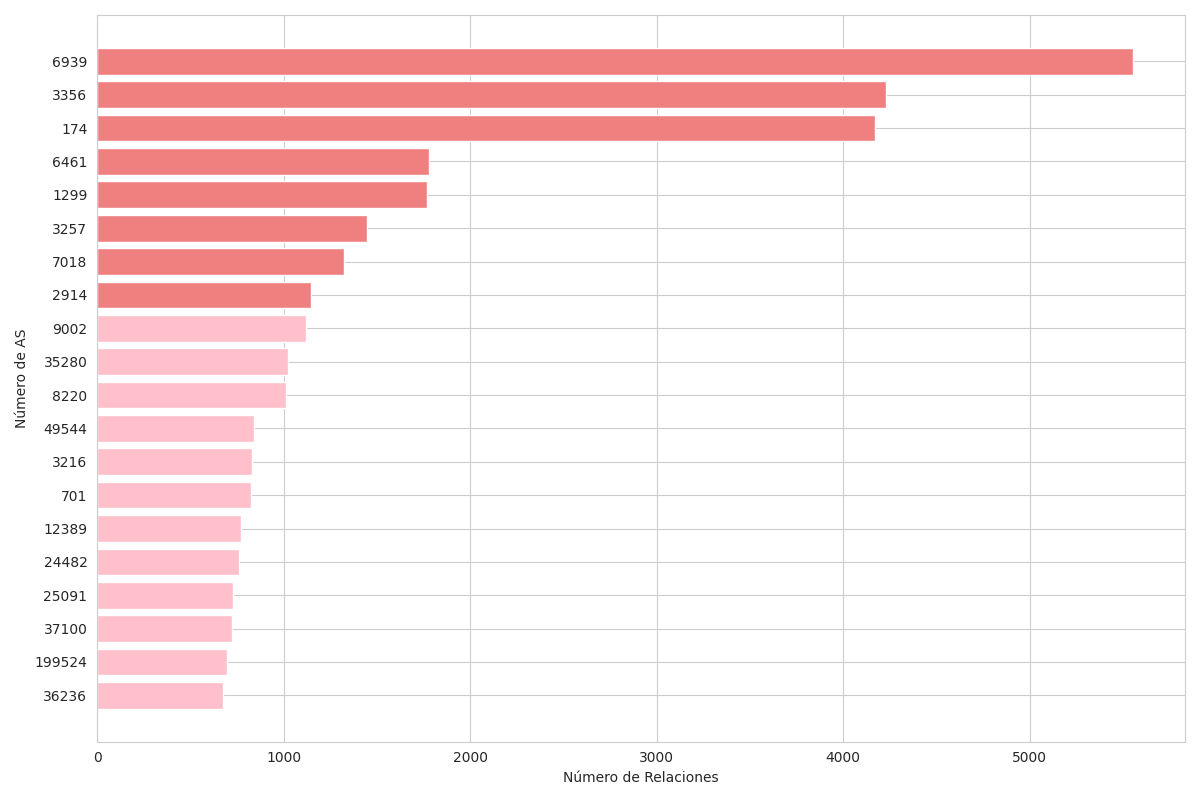
\includegraphics[width=0.9\textwidth]{img/resultados/top_20_as_febrero_numerorelaciones_src.png}
    \caption{Top 20 ASes con mayor número de conexiones (grado), para RIB de febrero 2024.}
\label{fig:top_20_as_febrero_numerorelaciones_src}
\end{figure}


La Figura~\ref{fig:distribucion_as_grado_salida_febrero_comparacion} muestra la distribución del grado de salida de los ASes en febrero, con y sin outliers. Este análisis se enfoca únicamente en las conexiones salientes, a diferencia del informe principal que considera el grado total (entradas y salidas).




\begin{figure}[H]
    \centering

    \begin{subfigure}[b]{0.48\textwidth}
        \centering
        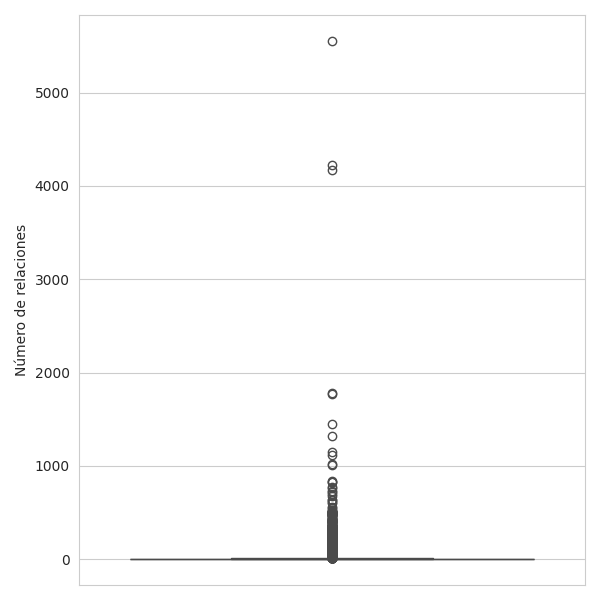
\includegraphics[width=\textwidth]{img/resultados/distribucion_as_grado_salida_febrero_boxplot_con_outliers.png}
        \caption{Con outliers.}
        \label{fig:distribucion_as_grado_salida_febrero_boxplot_con_outliers}
    \end{subfigure}
    \hfill
    \begin{subfigure}[b]{0.48\textwidth}
        \centering
        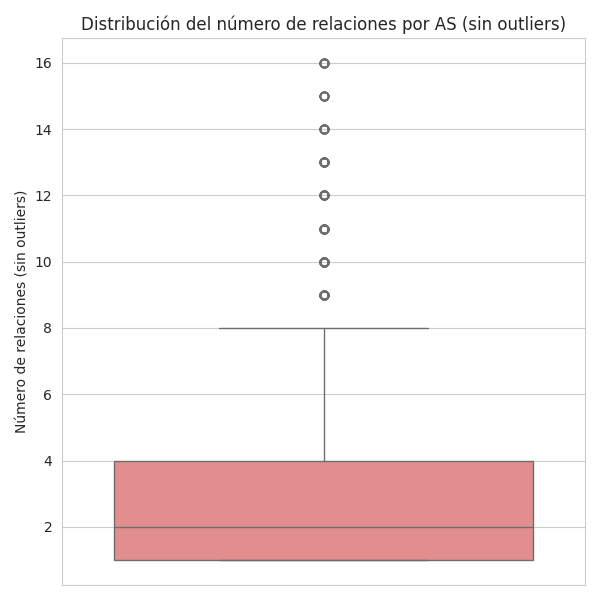
\includegraphics[width=\textwidth]{img/resultados/distribucion_as_grado_salida_febrero_boxplot_sin_outliers.png}
        \caption{Sin outliers.}
        \label{fig:distribucion_as_grado_salida_febrero_boxplot_sin_outliers}
    \end{subfigure}


    \caption{Comparación de la distribución del grado de salida de ASes en febrero, con y sin outliers.}
    \label{fig:distribucion_as_grado_salida_febrero_comparacion}
\end{figure}




La Figura~\ref{fig:comparacion_mensual_largo_paths} muestra la distribución de la longitud de las rutas BGP observadas durante los primeros cuatro meses del año 2024.


\begin{figure}[H]
    \centering
    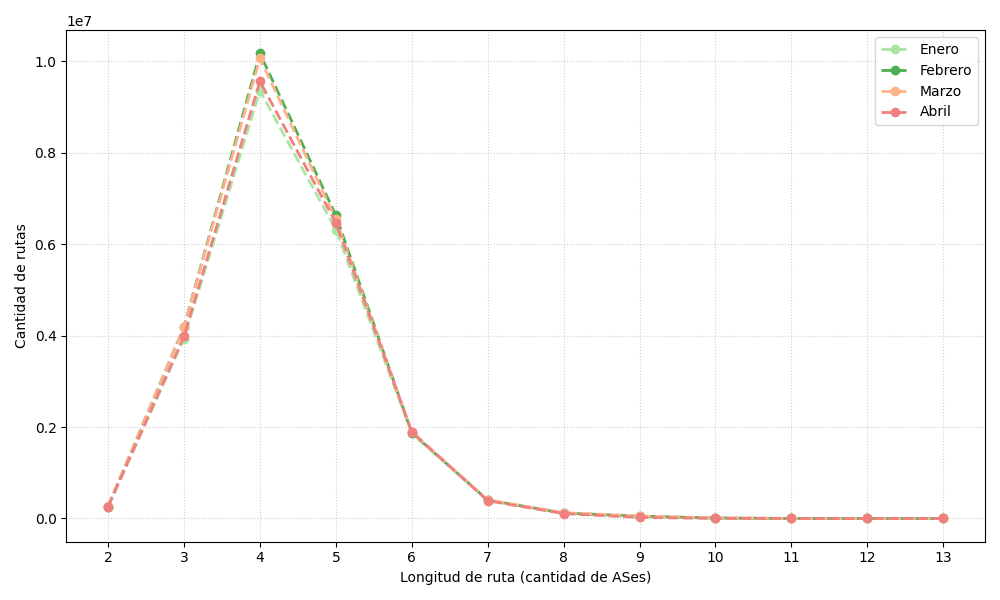
\includegraphics[width=0.8\textwidth]{img/resultados/comparacion_mensual_largo_paths.png}
    \caption{Comparación mensual de la longitud de rutas BGP.}
\label{fig:comparacion_mensual_largo_paths}
\end{figure}











\begin{table}[H]
\centering
\caption{Cantidad de ASes y aristas entre nodos en dataset de evaluacion asrank para los primeros 4 meses del ano}
\begin{tabular}{lcc}
\toprule
\textbf{Mes} & \textbf{Numero de ASes } & \textbf{Enlaces totales} \\
\midrule
Enero   &  76.351 & 499.651 \\
Febrero &  76.415 & 488.777 \\
Marzo   &  76.551 & 492.945 \\
Abril   &  76.644 & 495.601 \\
\end{tabular}
\label{tab:asrank_datasets}
\end{table}



\begin{table}[H]
\centering
\caption{Cantidad de ASes y aristas entre nodos en dataset de evaluacion asrank para los primeros 4 meses del ano}
\begin{tabular}{lcc}
\toprule
\textbf{Mes} & \textbf{Numero de ASes } & \textbf{Enlaces totales} \\
\midrule
Enero   &  76.351 & 499.651 \\
Febrero &  76.415 & 488.777 \\
Marzo   &  76.551 & 492.945 \\
Abril   &  76.644 & 495.601 \\
\end{tabular}
\label{tab:asrank_datasets}
\end{table}







